\documentclass[12pt]{article}
\usepackage[utf8]{inputenc}
\usepackage[main=russian,english]{babel}
\usepackage[left=20mm, top=15mm, right=20mm, bottom=10mm, nohead, nofoot]{geometry}

\usepackage{graphicx}
\usepackage{caption}
\usepackage{wrapfig}
\usepackage{multicol}
\usepackage{lipsum}
\usepackage{mwe}

% \def \var {value}
\newcommand{\ReportTheme}{Практика}
\newcommand{\ReportAuthor}{Данилевич Леонид, Лельчук Александр, 2022А класс}

\title{\bf \ReportTheme}
\author{\it \ReportAuthor}
\date{\today}

% 1. Титульный лист. (Одинаковая по форме. Взять в нетскуле)
% 2. Аннотация. (Около абзаца. Кратко, какая поставлена задача, какой результат получен. Делается в последний момент)
% 3. Оглавление.
% 4. Введение. (Где родилась задача. Ваша задача - подспорье в решении какой-то более глобальной. Зачем это всё нужно = Обоснование работы)
% 5. Постановка задачи. Сформулировать задачу так, чтобы можно было её решить математически/померить экспериментально/и т д.
% 6. Методика разрешения задачи. Как решается задача: математически/экспериментально/программно и т д. Подробности. С помощью каких механизмов.
% 7. Результаты. Что вы померили/насчитали/
% 8. Анализ результатов. Что означают результаты. Совпадают ли с предсказаниями. Что следует из результатов.
% 9. Список литературы. На что вы опирались.
% 10. Благодарности. С кем вы работали, кто вас консультировал, кто помогал и т п.

%\usepackage{mathptmx}

\begin{document}
   % \maketitle
   % титульный лист

    \begin{center}
    \large { {\bf Лицей «Физико-техническая школа»  Санкт-Петербургского Академического университета   } } 
    
    \vspace*{6\baselineskip}
    
    \large { {\bf Курсовая работа (отчет по практике) } } 
    
    \vspace*{6\baselineskip}
    
    Создание программы генериующей кроссворды из регулярных выражений \\
    \vspace*{3\baselineskip}
    
    \end{center}        
    \begin{flushright}
        Работу выполнили: \\
        Данилевич Леонид (2022А) \\
        Лельчук Александр (2022А) \\
        Научный руководитель: \\
        Дворкин Михаил Эдуардович \\
        Место прохождения практики: \\
        Лицей <<ФТШ>>
    \end{flushright}
    \vspace*{5\baselineskip}
    \begin{center}
        Санкт-Петербург, 2021
    \end{center}        
%----------------------------------------------------------------------------------------------------------
    \newpage % Аннотация
    
%----------------------------------------------------------------------------------------------------------
    \newpage % Оглавление
    { \center \bf Кроссворды из регулярных выражений }
\tableofcontents
%----------------------------------------------------------------------------------------------------------
    \newpage % Введение
\section{Введение}
Регулярные выражения — формальный язык поиска подстрок в тексте и манипуляций с ними. Например, регулярному выражению «.*amp(le)?» соответствуют строки «Sample», «example», «lamp» и некоторые другие. С помощью регулярных выражений можно достаточно просто искать в тексте подстроки определённого формата и заменять их на соответсвующие им другие подстроки. Новичкам, изучающим регулярные выражения, для закрепления нового материала полезно решить такой (https://gregable.com/p/regexp-puzzle.html) кроссворд (изображение ниже). Конкретно этот экземпляр создан, как задание конкурса «MIT Mystery Hunt» 2013 года. Мы решили написать приложение, автоматически генерирующее подобные кроссворды, а также позволяющее их решать. Мы считаем, что такое приложение будет полезно многим людям, изучающим регулярные выражения, а для знакомых с ними оно будет просто интересно.

%----------------------------------------------------------------------------------------------------------
    \newpage % Постановка задачи
     Необходимо разработать алгоритм генерации строк с различными паттернами, которые могли бы легко восприниматься человеком.
     И создать алгоритм генерации наиболее короткого регулярного выражения для задданной строки, а затем создать прилоожение на базе Android, реализующее этот функционал.


%----------------------------------------------------------------------------------------------------------
    \newpage % Методика решения задачи

\section{ Методика решения задачи: }
Так как задача состоит в написании программы, то решается программно. Задача дробится на части: 
\begin{enumerate} 
\item Собственно, решение уже имеющегося кроссворда. Понадобится для оценки сложности кроссворда и и удостоверения единственности решения.
\begin{enumerate} 
\item Для решения произвольного кроссворда необходимо разобрать(«распарсить») регулярные выражения, кодирующие его строчки. Для этого написана рекурсивная функция с запоминанием ответа (техника «мемоизации» динамического программирования), которая для заданного регулярного выражения и требуемой длины строчки находит в компактном виде всевозможные строчки, подходящие под данное выражение. Компактный вид обусловлен тем, что строчки состоят не из символов, а из битовых масок, где из любой маски можно выбрать любой символ и получить корректную строчку. «Обратные ссылки» (back references) в регулярных выражениях обрабатываются следующей техникой: два символа, запрашиваемые быть одинаковыми, соотвествуют одному и тому же битовому объекту-маске.
\item После разбора регулярных выражений кроссворд решается методом инкрементальных улучшений. Изначально каждой букве сопоставлена битовая маска, соответствующая всем символам алфавита. Алгоритм рассматривает все ещё не разгаданные буквы по порядку, сужая для каждой множество возможных значений. Существует вероятность встретить кроссворд, нерешаемый данной техникой. Однако для его разгадывания человеку потребуется долгий и утомительный перебор. Создание таких кроссвордов не входит в нашу задачу. В случае полного разгадывания кроссворда можно утверждать, что его решение существует и единственно.
\end{enumerate} 
\item Генерация буквенного заполнения кроссворда. Должны образовываться строчки, подходящие под различные регулярные выражения. Максимизируется красота заполнения — субъективное свойство, включающее в себя регулярность кроссворда, т. е. различные повторения подстрок и английские слова.
\begin{enumerate} 
\item Для генерации случайного поля, максимизирующего потенциальную оценку кроссворда, а именно, разнообразие типов регулярных выражений, разгадка необходимой степени сложности, и субъективная оценка красоты, применён метод имитации отжига («simulated annealing»). Большое количество итераций заменяют одну букву на изначально равномерно случайно сгенерированном поле, после чего в некотором случае изменение принимается, поле обновляется.
\end{enumerate} 
\item Генерация регулярных выражений, лучшим образом задающих получившиеся строчки.
\begin{enumerate} 
\item Пока не реализована
\end{enumerate} 
\item Оценка сложности, проверка единственности решения, путём программного решения
\begin{enumerate} 
\item Предполагается применять усреднённое значение количества итераций, требуемых алгоритму (1) для решения сгенерированного кроссворда при рассмотрении клеток, содержащих неразгаданные буквы, в случайном порядке
\end{enumerate} 
\end{enumerate} 


%----------------------------------------------------------------------------------------------------------
    \newpage % Результаты
    
\section{ Результаты }
        На рисунках ниже изображены ввод, предоставляемый нашей программе с консоли, и её вывод. Это кроссворд, упоминавшийся во введении, и можно убедиться, что он разгадан корректно.
    \begin{multicols}{2}
        \begin{figure*}[ht!]
            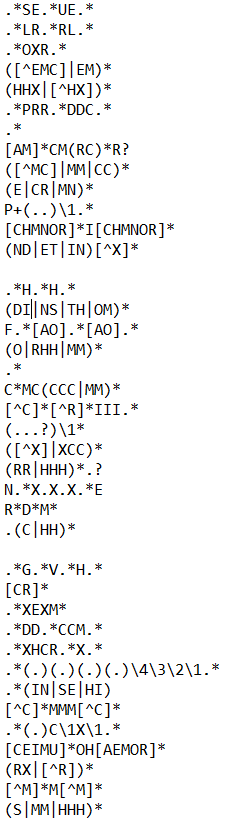
\includegraphics[width=.3\textwidth]{HexagonalInput1.PNG}\hfill
            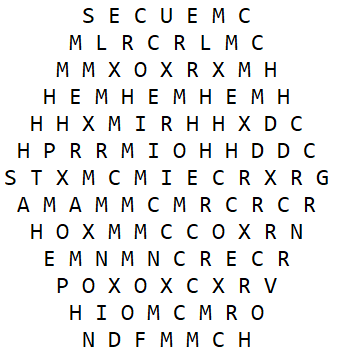
\includegraphics[width=.3\textwidth]{HexagonalOutput1.PNG}\hfill
            \caption{Регулярные выражения; ввод}
            \caption{Решение кроссворда нашей программой}
        \end{figure*}
    \end{multicols}
%----------------------------------------------------------------------------------------------------------
    \newpage % Анализ рез-ов
    Пока результаты не очень большие, но мы сделали многое из того, что хотели. \\
    Мы получили новый алгоритм, которого раньше не существовало, и который в перспективе может использоваться не только в наешм приложении, но также для генерации
    шаблонов для описания различных строк на основании только лишь одной входной строки. \\

    
%----------------------------------------------------------------------------------------------------------
%    \newpage % Список литры (у нас пуст в общем)

%----------------------------------------------------------------------------------------------------------
    \newpage % Благодарности

    Наш научный руководитель: { \bf Дворкин Михаил Эдуардович } \\
    \\
    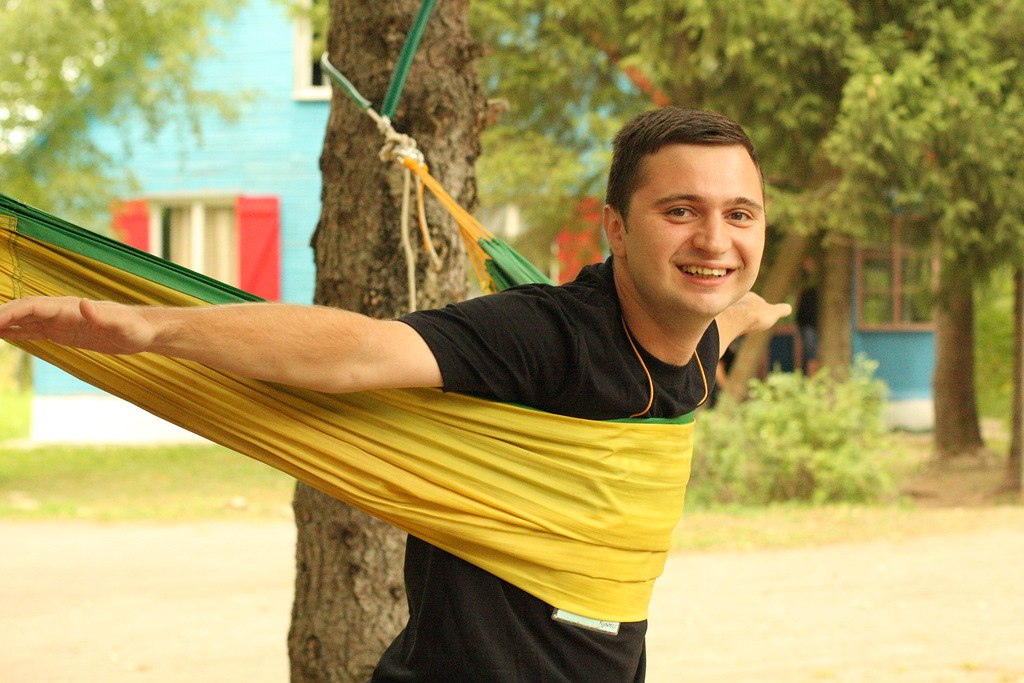
\includegraphics[scale=0.5]{dvorkin2.jpg}\hfill
    

        
\end{document}

